%%==================================================================%%
%% Author : Abascal Fern�ndez, Patricia                             %%
%%          S�nchez Barreiro, Pablo                                 %%
%% Version: 1.3, 18/06/2013                                         %%
%%                                                                  %%
%% Memoria del Proyecto Fin de Carrera                              %%
%% Antecedentes, archivo ra�z                                       %%
%%==================================================================%%

\chapterheader{Antecedentes y Planificaci�n}{Antecedentes y Planificaci�n}
\label{chap:background}

Este cap�tulo trata de describir a grandes rasgos las t�cnicas, tecnolog�as y herramientas utilizadas para el desarrollo del presente Proyecto Fin de Carrera. En primer lugar, se introducir� el caso de estudio que se utilizar� de forma recurrente a lo largo del proyecto. A continuaci�n, se describen diversos conceptos relacionados el dominio del proyecto, como son las l�neas de productos software, el desarrollo software orientado a caracter�sticas, la metodolog�a TENTE, el \emph{Slicer Pattern}, y las t�cnicas de generaci�n de c�digo. Se concluye con la planificaci�n que se ha llevado a cabo para la creaci�n del Proyecto.

\chaptertoc

\section{Caso de Estudio: Software para Hogares Inteligentes}
\label{sec:back:casoEstudio}

%%==========================================================================%%
%% Author : Sa�udo Olmedo, Ignacio                                          %%
%% Author : S�nchez Barreiro, Pablo                                         %%
%% Version: 1.2, 21/04/2014                                                 %%
%%                                                                          %%
%% Memoria del Proyecto Fin de Carrera                                      %%
%% M2M/Caso de estudio                                                      %%
%%==========================================================================%%

Como se explicaba en el capitulo 2 en la secci�n "Caso de estudio" el objetivo de este caso de estudio es la creaci�n de un generador de c�digo de una versi�n simplificada de Twitter.
En esta secci�n se reproducir�n los procesos M2M y M2T en el siguiente capitulo, todo esto bajo el proceso de desarrollo dirigido por modelos. Esta secci�n esta dedicada a describir la transformaci�n del modelo UML de Twissandra a un modelo Cassandra. Partiendo del modelo UML de la figura~\ref{back:fig:twissandra} y una vez establecidas las reglas de transformaci�n entre modelos, esta secci�n explica el proceso de transformaci�n del modelo UML al modelo Cassandra.

En primer lugar, marcamos el atributo username de la clase User como clave. En el caso de la clase FollowingRelationship y la clase Tweet al no tener un atributo marcado como clave generamos una clave sustituta autom�ticamente para cada clase, llamadas FollowingRelationship\_id y tweet\_id respectivamente.

Por cada paquete estereotipado como <<dataModel>>, se crea un nuevo keyspace. El nombre del keyspace ser� el nombre utilizado por el data model. Los atributos restantes de las meta-clases del keyspace se establecen en sus valores definidos por defecto. A continuaci�n, todos los elementos correspondientes de ese paquete se procesan y se colocan dentro de su keyspace correspondiente.

Como se mencionaba en las reglas de transformaci�n, la clase User se transforma en una Column Family llamada User. A continuaci�n, los atributos y las asociaciones se procesan. Por �ltimo, el atributo Username, que se marc� como clave en el modelo de datos UML, es marcado como Primary Key. De manera similar para aquellos atributos del modelo UML cuya multiplicidad sea igual a uno se realiza una transformaci�n simple, por ejemplo el atributo username y password se transforman en dos columnas, ambos del tipo text. Estas columnas est�n contenidas en la column family User. De la misma manera se transforman los atributos body y time de la clase Tweet y el atributo timestamp de la clase FollowingRelationship.
En el caso de el atributo del modelo UML email cuya multiplicidad es mayor de uno y tiene las propiedades isUnique establecida en false y la propiedad isOrdered establecida en false (en el modelo no se puede apreciar pero esta configurado as�), se transforma este atributo en un set llamado email de tipo text dentro de la column family User.

En cuanto a las asociaciaciones de multiplicidad igual a uno la transformaci�n que se realiza por ejemplo, para la asociaci�n de la clase user una nueva columna llamada user\_username (recordemos que username es la clave de la column family user) es creada y a�adida a la column family Tweet. Para las asociaciones cuya multiplicidad es mayor de uno, por ejemplo la asociaci�n llamada userline se crea una dynamic column family llamada User\_userline. A continuaci�n una columna llamada user\_username de tipo text es a�adida a esta column family. Despu�s una columna llamada tweet\_id de tipo uuid es a�adida (el atributo tweet\_id fue creado en la column family tweet al no tener clave). Las columnas user\_username y tweet\_id son designadas como primary key, la columna user\_username ser� la partition key. 

\section{L�neas de Producto Software}
\label{sec:back:spl}

%%==================================================================%%
%% Author : Abascal Fern�ndez, Patricia                             %%
%%          S�nchez Barreiro, Pablo                                 %%
%% Version: 1.3, 18/06/2013                                         %%
%%                                                                  %%
%% Memoria del Proyecto Fin de Carrera                              %%
%% Background/Software Product Lines                                %%
%===================================================================%%

El objetivo de una \emph{l�nea de producto software}~\cite{pohl:2010,kakola:2006} es crear una infraestructura adecuada a partir de la cual se puedan derivar, de forma tan autom�tica como sea posible, producto concretos pertenecientes a una familia de producto software. Una familia de producto software es un conjunto de aplicaciones software similares, lo que implica que comparten una serie de caracter�sticas comunes, pero que tambi�n presentan variaciones entre ellos.

Un ejemplo cl�sico de familia de producto software es el producto Parten�n, para software bancario, comentado en la introducci�n a este documento (ver Secci�n~\ref{sec:intr:introduction}). Dicho producto representa una familia de productos destinados a la gesti�n bancaria. Parten�n en s� no puede ser desplegado como una aplicaci�n, sino que necesita ser configurado de acuerdo a una serie de caracter�sticas concretas demandadas por cada cliente que require una instalaci�n de Parten�n.

La idea de una l�nea de producto software es proporcionar una forma autom�tica y sistem�tica de construir productos concretos dentro de una familia de producto software mediante la simple especificaci�n de qu� caracter�sticas deseamos incluir dentro de dicho producto. Esto representa una alternativa al enfoque tradicional de desarrollo software, el cual se basaba simplemente en seleccionar el producto m�s parecido, dentro de la familia, al que queremos construir y adaptarlo manualmente.

El proceso de creaci�n de l�neas de producto software se estructura dos fases: (1) \emph{Ingenier�a del Dominio} (en ingl�s,  \emph{Domain Engineering}); y (2) \emph{Ingenier�a de Aplicaci�n} (en ingl�s, \emph{Application Engineering}) (ver Figura~\ref{back:fig:domainAplicEng}). La \emph{Ingenier�a del Dominio} tiene como objetivo la creaci�n de la infraestructura o arquitectura de referencia de la l�nea de productos software. Esta arquitectura de referencia debe permitir la r�pida, o incluso autom�tica, construcci�n de sistemas software espec�ficos pertenecientes a la familia de productos software. La \emph{Ingenier�a de Aplicaci�n} utiliza la infraestructura creada anteriormente para crear aplicaciones espec�ficas adaptadas a las necesidades de cada usuario en concreto.

\begin{figure}[!tb]
  \centering
  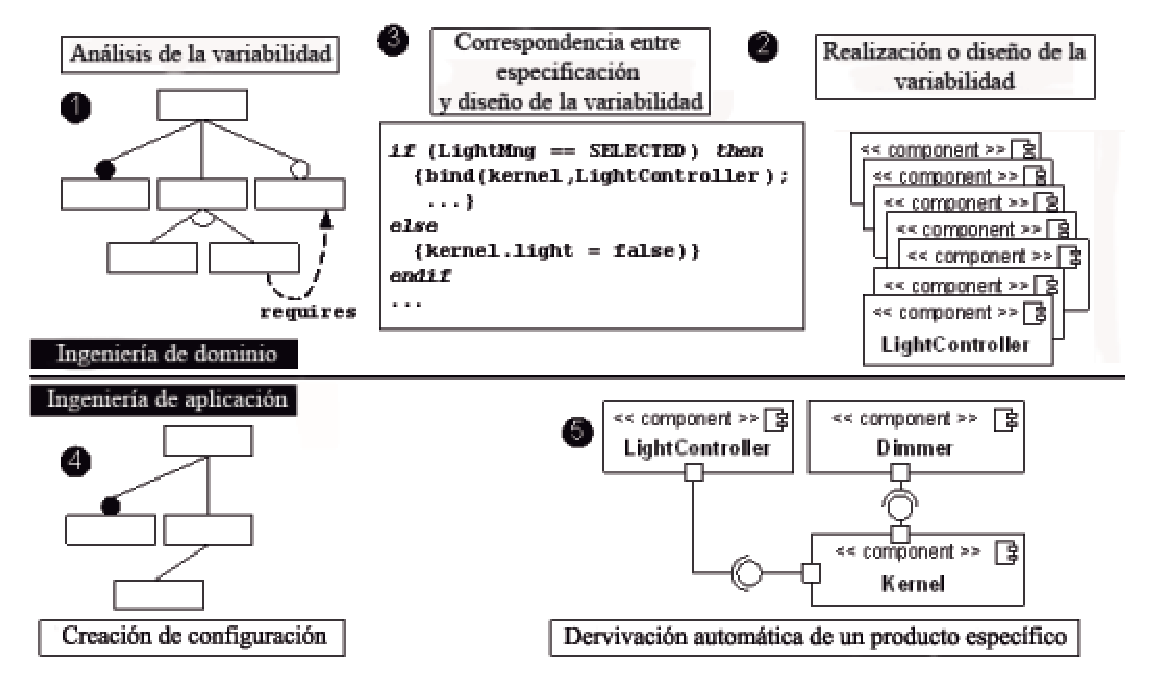
\includegraphics[width=.95\linewidth]{background/images/domainAplicationEngineering.eps} \\
  \caption{Proceso de Desarrollo de una l�nea de producto software}
  \label{back:fig:domainAplicEng}
\end{figure}

En la fase de Ingenier�a del Dominio, el primer paso a realizar es un an�lisis de qu� caracter�sticas de la familia de producto son variables y por qu� son variables. Esta parte es la que se conoce como \emph{An�lisis o Especificaci�n de la Variabilidad} (Figura~\ref{back:fig:domainAplicEng}, etiqueta 1).

A continuaci�n, se ha de dise�ar una arquitectura de referencia para la familia de producto software que permita soportar dicha variabilidad. Esta actividad se conoce como \emph{Realizaci�n o Dise�o de la Variabilidad} (Figura~\ref{back:fig:domainAplicEng}, etiqueta 2).

El siguiente paso es establecer una serie de reglas que especifiquen c�mo hay que instanciar o configurar la arquitectura previamente creada de acuerdo con las caracter�sticas seleccionadas por cada cliente. Esta fase es la que se conoce como \emph{Correspondencia entre Especificaci�n y Dise�o de la Variabilidad} (Figura~\ref{back:fig:domainAplicEng}, etiqueta 3).

Tras completar la fase de Ingenier�a del Dominio, disponemos de una especie de l�nea de montaje, la cual podemos utilizar para construir productos concretos de forma m�s o menos automatizada.

En la fase de Ingenier�a de Aplicaci�n, se crean productos concretos utilizando la infraestructura previamente creada. Para ello, el primer paso es crear una \emph{configuraci�n}, que no es m�s que una selecci�n de caracter�sticas que un usuario desea incluir en su producto concereto (Figura~\ref{back:fig:domainAplicEng}, etiqueta 4).

En el caso ideal, usando esta configuraci�n, se debe poder ejecutar las reglas de correspondencia entre especificaci�n y dise�o de la variabilidad para que la arquitectura creada en la fase de Ingenier�a del Dominio se adapte autom�ticamente; generando un producto concreto espec�fico acorde a las necesidades concretas del usuario (Figura~\ref{back:fig:domainAplicEng}, etiqueta 5). En el caso no ideal, dichas reglas de correspondencia deber�n ejecutarse a mano, lo cual suele ser un proceso tedioso, largo, repetitivo y propenso a errores.

La siguiente secci�n describe el paradigma de desarrollo software orientada a caracter�sticas, el cual est� �ntimamente ligado al dise�o e implementaci�n de l�neas de productos software.



\section{Dise�o Orientado a Caracter�sticas con UML}
\label{sec:back:uml}

%%==================================================================%%
%% Author : Abascal Fern�ndez, Patricia                             %%
%%          S�nchez Barreiro, Pablo                                 %%
%% Version: 1.1, 18/06/2013                                         %%
%%                                                                  %%
%% Memoria del Proyecto Fin de Carrera                              %%
%% Background/Dise�o Orientado a Caracter�sticas con UML            %%
%===================================================================%%

El \emph{dise�o orientado a caracter�sticas}~\cite{kastner:2008} es un paradigma para la construcci�n, adaptaci�n y s�ntesis de sistemas software a gran escala. Una \emph{caracter�stica} es una unidad coherente funcionalidad de un sistema software. Una caracter�sticas proporciona una opci�n de configuraci�n potencial, ya que dicha caracter�stica debe poder ser incluida o excluida del producto software, dando lugar a productos software con diferentes funcionalidades. Por ejemplo, en el caso del software de gesti�n de hogares inteligentes, toda la funcionalidad relacionada con la gesti�n autom�tica de luces, ser�a considerada como una caracter�stica.

La idea b�sica del dise�o orientado a caracter�sticas es descomponer un sistema software en m�dulos bien definidos, donde cada m�dulo encapsula una caracter�stica que el sistema ofrece. El objetivo de la descomposici�n es la construcci�n de software bien estructurado que puede ser adaptado a las necesidades del usuario y el entorno, mediante la selecci�n y composici�n de las caracter�sticas adecuadas.

Por tanto, a partir de un conjunto de caracter�sticas, se pueden generar multitud de sistemas software compartiendo caracter�sticas comunes y diferenci�ndose en otras, lo que hace que este paradigma sea especialmente adecuado para el dise�o e implementaci�n de \emph{l�nea de productos software}.

Para ilustrar como funciona el paradigma orientado a caracter�sticas, utilizaremos un dise�o UML  (ver Figura~\ref{back:fig:smartHome}) orientado a caracter�sticas ilustraremos de nuestro caso de estudio, el software de gesti�n de hogares inteligentes~\ref{sec:back:casoEstudio}. Por razones de claridad, se ha simplificado dicho modelo de dise�o, eliminando ciertas operaciones de la clase \emph{Gateway} y suprimiendo todas las clases relacionadas con la interfaz gr�fica de usuario.

Dos conceptos com�nmente utilizados por los lenguajes orientados a caracter�sticas son el concepto de \emph{familia de clases} y de \emph{clase virtual}.

\begin{figure}[!tb]
  \centering
  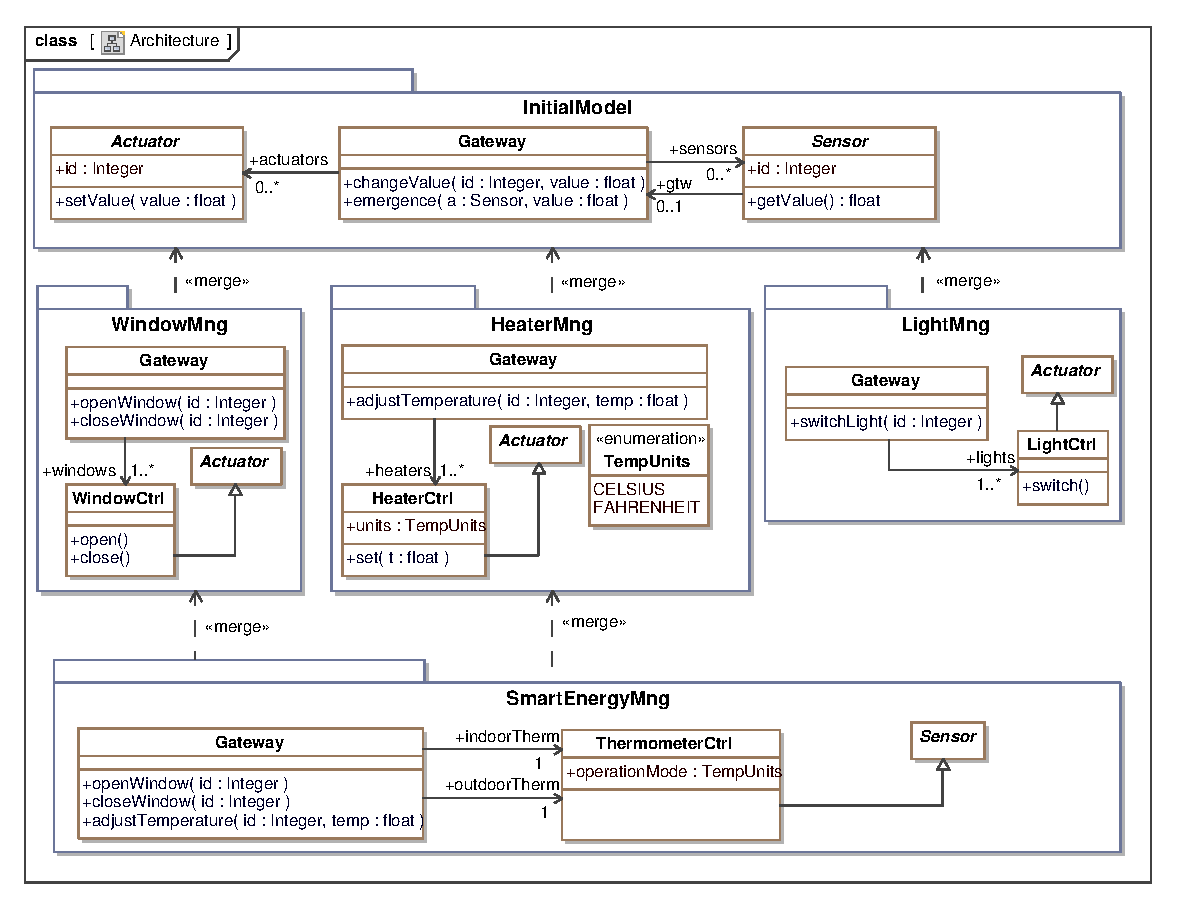
\includegraphics[width=\linewidth]{background/images/umlDesign.eps} \\
  \caption{Dise�o orientado a caracter�sticas del software para hogares inteligentes}
  \label{back:fig:smartHome}
\end{figure}

Una \emph{familia de clases} es un nuevo tipo de m�dulo que se utiliza para encapsular y gestionar como una unidad de composici�n un conjunto de clases pertenecientes a una misma caracter�stica. Por ejemplo, en nuestro caso de estudio, todas las clases que est�n relacionadas con la gesti�n autom�ticas de luces, deber�an estar encapsuladas en una misma familia de clases. Estas familias de clases se representan en el modelo UML de la Figura~\ref{back:fig:smartHome} como paquetes que contienen clases. Por ejemplo, el paquete \emph{LightMng} representa la familia de clases que se corresponder�a con la caracter�stica \emph{gesti�n de luces autom�ticas}.

Una \emph{clase virtual} es una clase perteneciente a una familia de clases y que es susceptible de ser heredada y sobreescrita por familias de clases, al estilo de los m�todos virtuales de una clase en el paradigma orientado a objetos~\citep{madsen:1989}.

La herencia entre familias de clases se representa en nuestro modelo UML mediante relaciones \emph{merge}, de acuerdo a la t�cnica expuesta por~\cite{laguna:2010}. Cuando una familia de clases hereda de otra, hereda impl�citamente todas sus clases virtuales. Todas las clases de una familia de clases son impl�citamente clases virtuales.

Si una clase estuviese presente tanto en una familia de clases padre como en una familia de clases hija, como por ejemplo, \imp{Gateway} en \imp{LightMng} y \imp{BaseSystem} en la Figura~\ref{back:fig:smartHome}, el resultado que se produce es el mismo que se producir�a si la clase virtual perteneciente a la familia de clases hija, heredase de la clase virtual perteneciente a la familia de clases padre. Por ejemplo, en nuestro caso, la aplicaci�n funcionar�a como si clase \imp{Gateway} de \imp{LightMng} heredase de la clase \imp{Gateway} de \imp{BaseSystem}.

De este modo, una clase virtual de una familia de clases hija, puede a�adir nuevos atributos y m�todos a las clases virtuales de las familias de clases padre. De igual forma, se pueden sobreescribir m�todos de las virtuales de las familias de clases padre. Se�alar que la herencia m�ltiple entre familias de clases s� suele estar permitida y soportada en los lenguajes de programaci�n orientados a caracter�sticas.

%%=======================================================================%%
%% NOTA(Pablo): Esto es demasiado t�cnico y en realidad no se utiliza    %%
%%              en tu proyecto, aunque es una de las grandes ventajas    %%
%%              de CaesarJ.                                              %%        %%=======================================================================%%
%%
%% Adem�s, las referencias entre clases se actualizan autom�ticamente.
%% Por ejemplo, en el caso de la figura~\ref{back:fig:smartHome}, aunque
%% no se haga expl�citamente, cualquier referencia a una clase del tipo
%% \imp{Gateway} dentro de la familia de clases \imp{LightMng} se
%% referir� a la clase virtual \imp{Gateway} de la familia de clases
%% \imp{LightMng} y no a la clase virtual de mismo nombre de la familia
%% de clases \imp{BaseSystem}. De esta forma, las referencias est�n
%% siempre actualizadas a su versi�n m�s extendida.
%%
%%
%%=======================================================================%%

Para implementar una l�nea de productos software, cada caracter�stica se tiende a manipular como una familia de clases. Dentro de cada familia de clases, cada caracter�stica se dise�a usando las t�cnicas tradicionales de la orientaci�n a objetos, tal como se muestra en la figura~\ref{back:fig:smartHome}.

Por �ltimo, comentar que no todas las caracter�sticas pueden ser correctamente implementadas como familia de clases. Por ejemplo, en nuestro ejemplo, una caracter�stica del sistema es el modo de operaci�n de los aparatos de fr�o/calor, los cuales pueden funcionar en grados Celsius o Fahrenheit. Este tipo de variabilidad se implementa mejor introduciendo un par�metro de configuraci�n en las clases que corresponda, que creando familias de clases separadas para cada opci�n. No obstante, los lenguajes de programaci�n orientados a caracter�sticas no impiden la utilizaci�n de los mecanismos tradicionales de gesti�n de la variabilidad de los lenguajes orientados a objetos, como la parametrizaci�n o los patrones de dise�o~\citep{loughran:2008}.

Para realizar una configuraci�n, es decir, para crear un producto concreto por composici�n de caracter�sticas, simplemente hay que crear una nueva familia de clases que herede de las familias de clases que correspondan a las caracter�sticas seleccionadas. Por ejemplo, si quisi�ramos crear un producto concreto que tuviese las caracter�sticas \imp{LightMng} y \imp{WindowMng}, crear�amos una familia de clases, la cual estar�a vac�a, y la que le damos como nombre, por ejemplo, \imp{PatriciaHouse}. A continuaci�n, hacemos que \imp{PatriciaHouse} herede de \imp{LightMng} y \imp{WindowMng}. De esta forma, ambas caracter�sticas se combinan en la familia de clases hija, la cual representar�a un producto concreto con dichas caracter�sticas. Por tanto, el proceso de composici�n de caracter�sticas, se realiza mediante herencia entre familias de clases.

La siguiente secci�n proporciona una breve descripci�n sobre la metodolog�a TENTE, una metodolog�a orientada a caracter�sticas y dirigida por modelos para el desarrollo y configuraci�n de l�neas de productos software.



\section{TENTE}
\label{sec:back:tente}

%%==================================================================%%
%% Author : Abascal Fern�ndez, Patricia                             %%
%%          S�nchez Barreiro, Pablo                                 %%
%% Version: 1.1, 18/06/2013                                         %%
%%                                                                  %%
%% Memoria del Proyecto Fin de Carrera                              %%
%% Background/TENTE                                                 %%
%===================================================================%%

TENTE~\cite{fuentes:2009:caise,sanchez:2011:tente} es una moderna metodolog�a para el desarrollo de l�neas de productos software desarrollada en el contexto del proyecto AMPLE\footnote{www.ample-project.net}. TENTE integra diversos avances para el desarrollo de l�neas de productos software, tales como avanzadas t�cnicas de modularizaci�n y desarrollo software dirigido por modelos.

Las t�cnicas avanzadas de modularizaci�n permiten el encapsulamiento en m�dulos bien definidos y f�cilmente componibles de las diferentes caracter�sticas de una familia de productos software, lo cual simplifica el proceso de construcci�n de productos espec�ficos. Dicha modularizaci�n de caracter�sticas se realiza desde la fase arquitect�nica, usando mecanismos espec�ficos del lenguaje de modelado UML~\cite{uml:2005}.

Despu�s, mediante el uso de generadores de c�digo, a partir del dise�o arquitect�nico de una familia de productos software se genera el esqueleto de su implementaci�n. Dicha implementaci�n se realiza en el lenguaje \emph{CaesarJ}~\cite{aracic:2006}, una extensi�n de Java que incluye potentes mecanismos para soportar la separaci�n y composici�n de caracter�sticas.

Dichos esqueletos se han de completar manualmente, obteni�ndose al final un conjunto de m�dulos software, o piezas, cuya composici�n da lugar a productos software concretos\footnote{El nombre de la metodolog�a proviene del c�lebre juego de construcci�n TENTE, versi�n espa�ola del popular Lego, el cual permite realizar diferentes construcciones mediante el ensamblado de una serie de piezas predefinidas}. Dichos m�dulos constituyen lo que se conoce como la implementaci�n de referencia de la l�nea de productos software.

Para la derivaci�n de productos concretos desde la infraestructura descrita en el p�rrafo anterior, TENTE usa un innovador lenguaje, denominado VML (\emph{Variability Management Language})~\cite{loughran:2008,sanchez:2008} para la especificaci�n de las reglas que indican c�mo se ha de configurar una arquitectura de referencia de acuerdo con la selecci�n de caracter�sticas de cada cliente en particular.

Posteriormente, a nivel de Ingenier�a de Aplicaciones (ver Figura~\ref{back:fig:domainAplicEng}), se crea un modelo de configuraci�n, el cual debe contener una lista con las caracter�sticas que el cliente desea incluir o excluir de su producto concreto. Utilizando este modelo de configuraci�n como entrada, VML es capaz de ejecutar las reglas de derivaci�n anteriormente especificadas para crear de forma autom�tica el modelo de la arquitect�nico del producto deseado por el cliente.

A continuaci�n, se utiliza dicho modelo de un producto concreto como entrada para un generador autom�tico de c�digo, que crear� el c�digo necesario para componer los m�dulos o piezas software pertenecientes a la implementaci�n de referencia de la l�nea de productos software.

Esta metodolog�a posee diversas ventajas:

\begin{enumerate}
	\item Gracias al uso de t�cnicas orientadas a caracter�sticas, como el operador \emph{merge} de UML y el lenguaje CaesarJ, se facilita la modularizaci�n y composici�n de caracter�sticas, lo que facilita no s�lo el proceso de obtenci�n de productos concretos, sino tambi�n la reutilizaci�n y evoluci�n de dichas caracter�sticas~\cite{figueiredo:2008}.
	\item Gracias al uso de t�cnicas dirigidas por modelos, se automatiza gran parte del proceso, evitando tareas repetitivas, largas, tediosas y mon�tonas, usualmente propensas a errores.
\end{enumerate}

No obstante, a pesar de sus bondades, se han encontrado diversas dificultades a la hora de transferir esta metodolog�a a las empresas de desarrollo software pertenecientes al tejido industrial c�ntabro.

Tal como se ha comentado anteriormente, TENTE est� dise�ado, para utilizar como lenguaje de programaci�n \emph{CaesarJ}. No obstante, la mayor�a de las empresas son bastante reticentes a cambiar su lenguaje habitual de programaci�n, por la razones ya expuestas (ver Secci�n~\ref{sec:intr:introduction}).

Fue por ello, junto con la preferencia de la mayor�a de las empresas de desarrollo software c�ntabras por la plataforma .NET, por lo que se decidi� desarrollar la metodolog�a Te.Net (ver Secci�n~\ref{sec:intr:tenet}).

El primero paso, tal como se ha comentado previamente, fue dise�ar un mecanismo que permitiese simular las ventajas de los lenguajes orientados a caracter�sticas en C\#. Dicho mecanismo, conocido como el \emph{Slicer Pattern}, se describe en la siguiente secci�n.




\section{Slicer Pattern}
\label{sec:back:slicer}

%%==================================================================%%
%% Author : Abascal Fern�ndez, Patricia                             %%
%%          S�nchez Barreiro, Pablo                                 %%
%% Version: 1.3, 18/06/2013                                         %%
%%                                                                  %%
%% Memoria del Proyecto Fin de Carrera                              %%
%% Background/Slicer Pattern                                        %%
%===================================================================%%

El mecanismo utilizado por la metodolog�a Te.Net para gestionar la variabilidad de una l�nea de productos a nivel de c�digo es el \emph{Slicer Pattern}~\cite{perez:2011}. Dicho patr�n se basa fuertemente en el concepto de clases parciales existente en C\#. Por tanto, antes de proceder a la descripci�n de dicho patr�n, introduciremos al lector en el concepto de clase parcial. M�s concretamente, nos centraremos en el concepto de clase parcial proporcionado por C\#.

\subsection{Clases Parciales C\#}

Las clases parciales de C\#~\cite{albahari:2010} permiten dividir la implementaci�n de una clase en varios archivos de c�digo fuente. Cada fragmento representa una parte de la funcionalidad global de la clase. Todos estos fragmentos se combinan, en tiempo de compilaci�n, para crear una �nica clase, la cual contiene toda la funcionalidad especificada en las clases parciales.

Por lo tanto, las clases parciales C\# parecen un mecanismo adecuado para implementar caracter�sticas, tal como ha sido identificado por diversos autores~\cite{laguna:2007,laguna:2010}. La idea es que cada incremento en funcionalidad perteneciente a una caracter�stica se podr�a encapsular en una clase parcial separada. Cuando un cliente solicita un producto con una serie de caracter�sticas concretas, se combinar�an (compilar�an) las clases parciales correspondientes a esas caracter�sticas. Esto dar�a lugar a un producto que contendr�a �nica y exclusivamente las caracter�sticas seleccionadas.

Ilustramos esta idea con un ejemplo basado en el caso de estudio del presente proyecto, expuesto en la Figura~\ref{back:fig:smartHome}. La Figura~\ref{back:code:partialClasses} muestra un ejemplo donde las clases parciales se aplican a la implementaci�n de la clase \imp{Gateway}. La implementaci�n de esta clase para las caracter�siticas \imp{BaseSystem} y \imp{LightMng} ha sido separada en dos ficheros (Figura~\ref{back:code:partialClasses} l�neas 0-9 y l�neas 10-15) con el mismo nombre, pero emplazados en distintos directorios (\imp{BaseSystem/Gateway.cs} y \imp{LightMng/Gateway.cs}). 

La clase \imp{Gateway} para la caracter�stica \imp{BaseSystem} (Figura~\ref{back:code:partialClasses} l�neas 0-9) contiene colecciones para sensores y actuadores (l�neas 2 y 3), al igual que los m�todos \imp{changeValue}, \imp{emergence} (l�neas 5-6), acorde al modelo de la Figura~\ref{back:fig:smartHome}. La clase \imp{Gateway} para la caracter�stica \imp{LightMng} (Figura~\ref{back:code:partialClasses} l�neas 10-15) contiene la colecci�n \imp{ligthCtrl} (l�nea 12) y el m�todo \imp{switchLigth} (l�nea 14).

\begin{figure}[!tb]
\begin{center}
\begin{footnotesize}
\begin{verbatim}
File BaseSystem/Gateway.cs
--------------------------------------------------------
0 namespace SmartHome {
1    public partial class Gateway {
2       protected IList<Sensor> sensors;
3       protected IList<Actuator> actuators;
4
5       private void changeValue(Int id, float value) {...}
6       private void emergence(Sensor a, float value) {...}
7    }
8 }

File LightMng/Gateway.cs
--------------------------------------------------------
10 namespace SmartHome {
11     public partial class Gateway {
12        private ISet<LigthCtrl> ligthCtrl;
13
14        private void switchLight(Int id) {...}
15 }

File SmartHome.csproj
--------------------------------------------------------
16 </Project>
17 ...
18 <ItemGroup>
19 <Compile Include="BaseSystem\Gateway.cs" />
20 <Compile Include="LightMng\Gateway.cs" />
21 <!-- 
22 <Compile Include="HeaterMng\Gateway.cs" />
23 <Compile Include="WindowMng\Gateway.cs" />
24 <Compile Include="SmartEnergyMng\Gateway.cs" />
25 -->
26 ...
27 </ItemGroup>
28 </Project>
\end{verbatim}
\end{footnotesize}
\end{center}
\caption{Implementaci�n de la clase \imp{Gateway} usando clases parciales}
\label{back:code:partialClasses}
\end{figure}

La Figura~\ref{back:code:partialClasses} (l�neas 16-28) muestra el fichero de construcci�n o compilaci�n (\imp{SmartHome.csproj}) para este proyecto. Ese fichero indica que las clases parciales para las caracter�sticas \imp{BaseSystem} y \imp{LightMng} est�n incluidas en la unidad de compilaci�n; pero las correspondientes clases parciales para las caracter�sticas \imp{HeaterMng}, \imp{WindowMng} y \imp{SmartEnergyMng} deben ser excluidas. Por tanto, el compilador generar� una clase \imp{Gateway} con la funcionalidad para controlar las luces pero no para controlar las ventanas o las temperaturas.

Inicialmente, las clases parciales de C\# parecen un mecanismo adecuado para dar soporte a la orientaci�n a caracter�sticas, al permitir dividir una clase en varias porciones, cada una de ellas correspondientes con una caracter�stica del producto a implementar.

Sin embargo, de acuerdo a una serie de experimentos realizados por~\cite{sanchez:2010} y \cite{perez:2011}, las clases parciales poseen una serie inconvenientes que necesitan ser resueltos para que puedan ser utilizadas para implementar caracter�sticas. El principal problema es que utilizando clases parciales, no podemos ni sobreescribir ni extender m�todos ya existentes dentro de una clase parcial. Ilustramos este problema con un ejemplo.

De acuerdo al modelo de la Figura~\ref{back:fig:smartHome} cuando se implementa la caracter�stica \imp{LightMng}, debemos a�adir una nueva colecci�n, llamada \imp{LightCtrl}, para almacenar objetos de tipo \imp{LightCtrl} para la clase \imp{Gateway}. Sin embargo, debemos tambi�n extender el contructor de la clase \imp{Gateway} para inicializar apropiadamente dicha colecci�n.

\begin{figure}[!tb]
\begin{center}
\begin{footnotesize}
\begin{verbatim}
File BaseSystem/Gateway.cs
--------------------------------------------------------
1 public partial class Gateway {
2 ...
3    public Gateway() {
4       this.floors = new List<Floor>();
5       this.interfaces = new List<CentralGUI>();
6    }
7 }
File LightMng/Gateway.cs
--------------------------------------------------------
8 public partial class Gateway {
9
10    protected IList<LightCtrl> lightCtrl;
11
12    public Gateway() {
13       this.lightCtrl = new List<LightCtrl>();
14    }
15 }
\end{verbatim}
\end{footnotesize}
\end{center}
\caption{Implementaci�n del constructor de la clase \imp{Gateway} usando clases parciales}
\label{back:code:constructor}
\end{figure}

Siguiendo esta argumentaci�n, se intenta escribir el c�digo descrito en la Figura~\ref{back:code:constructor}. Dicho c�digo contiene el constructor de la clase \imp{Gateway} para la caracter�stica \imp{BaseSystem} (Figura~\ref{back:code:constructor}, l�neas 3-6). Este constructor deber�a poder ser extendido en la clase parcial \imp{Gateway} de la caracter�stica \imp{WindowMng} tal como se muestra en la  Figura~\ref{back:code:constructor}, l�neas 10-12.

Sin embargo, esto no es posible puesto que el compilador reporta un error indicando que el m�todo \imp{Gateway()} est� duplicado y hay ambig�edad. Esto significa que no podemos separar la implementaci�n de un m�todo en varios archivos, ya que no se puede tener m�todos con el mismo nombre en dos clases parciales distintas. Esto reduce las capacidades de extensi�n proporcionadas por las clases parciales a la adici�n de nuevos m�todos y atributos, siendo imposible a�adir funcionalidad o sobreescribir m�todos existentes. 

Por ejemplo, el caso de la caracter�stica \imp{SmartEnergyMng}, la clase parcial \imp{Gateway} debe sobreescribir el m�todo \imp{adjustTemperature} de la clase \imp{Gateway} de la caracter�stica \imp{HeaterMng} para comprobar si las ventanas deben cerrarse antes de cambiar la temperatura de los aparatos de fr�o calor. No obstante, como no podemos a�adir un m�todo \imp{adjustTemperature} a la clase parcial \imp{Gateway} de la caracter�stica \imp{SmartEnergyMng} con el mismo nombre que el declarado en la caracter�stica \imp{HeaterMng}, no hay forma de sobreescribir el m�todo.

El \emph{Slicer Pattern} surge como soluci�n para resolver estas limitaciones. Dicho patr�n se describe en la siguiente subsecci�n.

\subsection{\emph{Slicer Pattern}}

El \emph{Slicer Pattern} se basa en la siguiente idea: dado que el problema es que no pod�amos tener m�todos con el mismo nombre en diferentes clases parciales, la soluci�n consiste en a�adir un prefijo a cada m�todo, de forma que cada m�todo tenga un nombre diferente. Dicho prefijo ser� el nombre de la caracter�sticas a la cual pertenece la clase parcial que contiene cada m�todo.

La Figura~\ref{back:fig:slicerPattern} muestra un ejemplo de dise�o para el hogar inteligente, el cual ha sido realizado siguiendo esta idea. 

\begin{figure}[!tb]
  \centering
  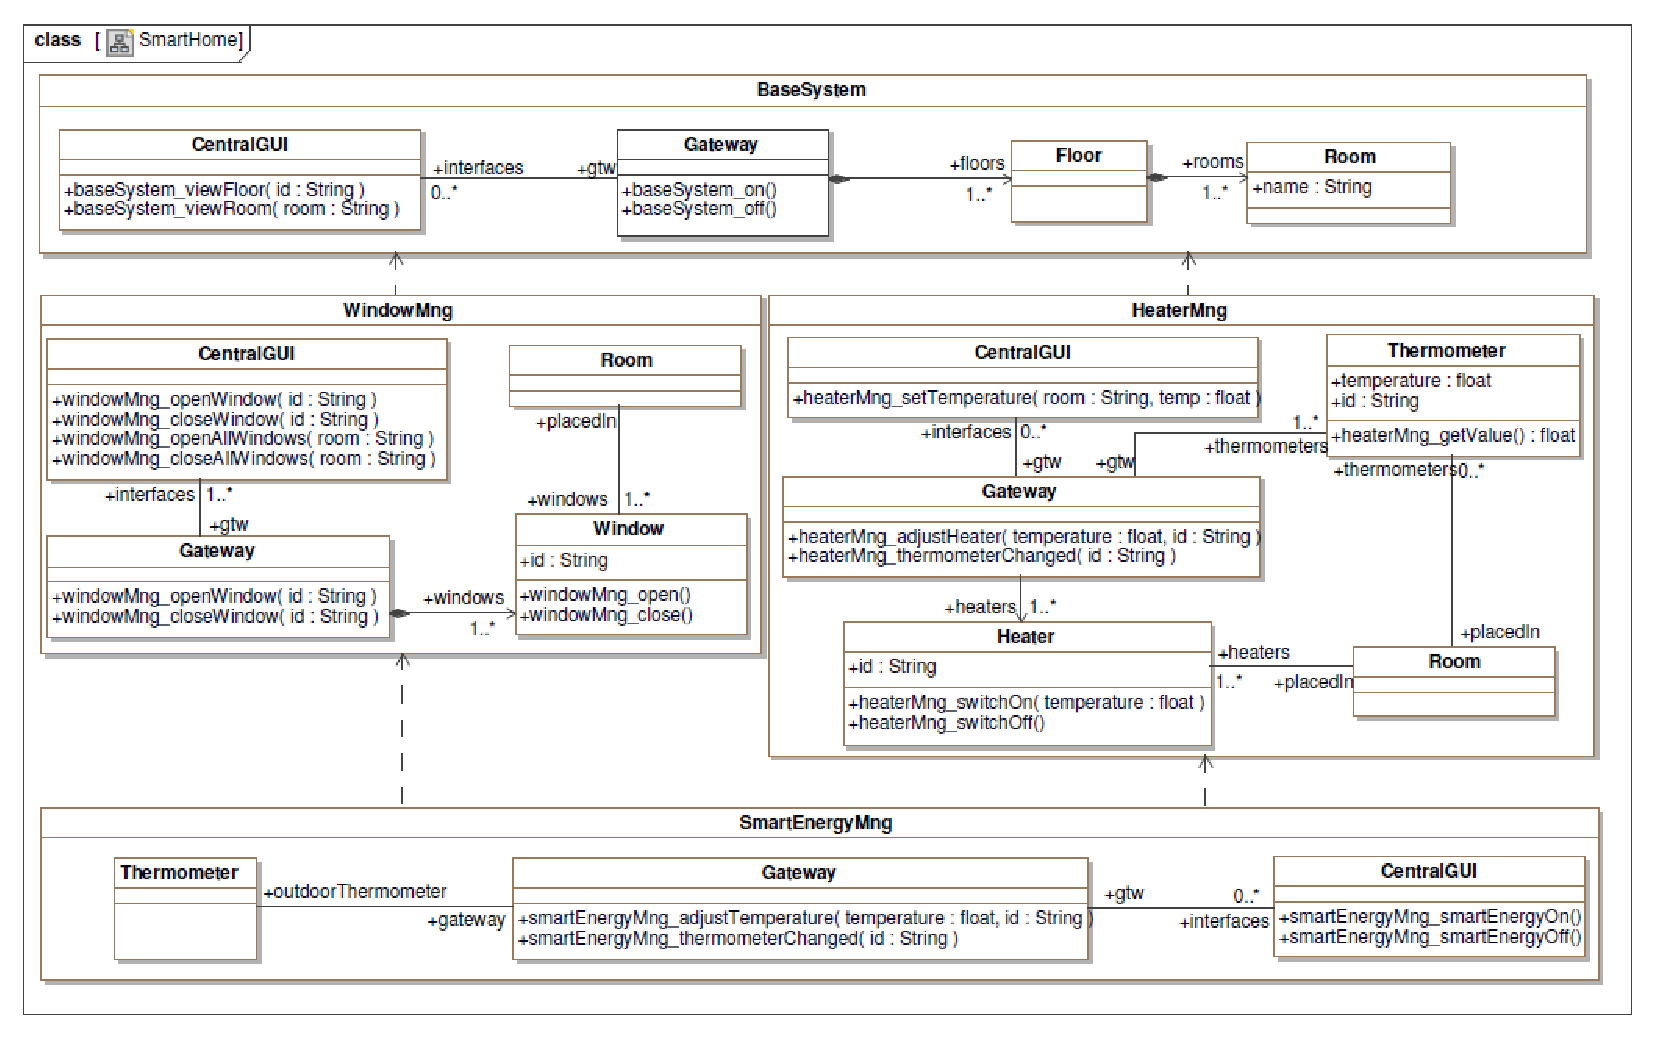
\includegraphics[width=.95\linewidth]{background/images/slicerPattern.eps} \\
  \caption{Proceso de Desarrollo de una L�nea de Productos Software}
  \label{back:fig:slicerPattern}
\end{figure}

Usando esta estrategia se puede comprobar c�mo, por ejemplo, las versiones del m�todo \imp{thermometerChanged} correspondientes a las caracter�sticas \imp{HeaterMng} y \imp{SmartEnergyMng} han sido transformadas en \imp{heaterMng\_thermometerChanged} y \imp{smartEnergyMng\_thermometerChanged} respectivamente y por tanto pueden co-existir sin que sus nombres colisionen. Es m�s, el m�todo \imp{smartEnergyMng\_thermometerChanged} puede extender del m�todo \imp{heaterMng\_thermometerChanged}. Se dispone por tanto de varias versiones parciales de un mismo m�todo. A las versiones prefijadas de un m�todo les denominaremos \emph{versiones sucias} de dicho m�todo.

Para generar un producto espec�fico es necesario que, a nivel de Ingenier�a de Aplicaci�n, se compongan o combinen dichas versiones sucias. Para ello, cada vez que queramos configurar una nueva aplicaci�n, debemos crear, por cada clase que deba ser incluida en el producto final, una nueva clase parcial, la cual se encargar� de combinar o componer dichos m�todos sucios de las clases parciales correspondientes a caracter�sticas. Dicha clase parcial contendr�a lo que denominaremos la \emph{versi�n limpia} de los m�todos a componer, es decir, las versiones de los m�todos sin prefijar, que ser�an adem�s p�blicos.

En nuestro caso, para configurar la clase \emph{Gateway} con control inteligente de la energ�a, se crear�a una nueva clase parcial \emph{Gateway}. Dicho m�todo contendr�a, por ejemplo, el m�todo \imp{thermometerChanged} (sin prefijo alguno). 

A continuaci�n, para componer los m�todos, se hace que cada m�todo limpio \emph{delegue} en tantos m�todos sucios como fuere necesario, de acuerdo a las caracter�sticas seleccionadas para el producto que se est� construyendo. En nuestro caso, \imp{thermometerChanged} delegar�a en \imp{smartEnergy\_thermometerChanged}.

Para evitar que los m�todos sucios \imp{heaterMng\_thermometerChanged} y \imp{smartEnergyMng\_thermometerChanged} puedan ser invocados directamente por objetos que no sean de la clase \imp{Gateway}, todas las versiones sucias de un m�todos ser�n privadas. De esta forma, s�lo son invocables las versiones limpias de un m�todo.

Esta idea, tal cual, no puede utilizarse para los constructores de la clases, ya que dichos constructores no se pueden ser renombrados, al tener que seguir un patr�n espec�fico para su nombre. Por tanto, necesitamos utilizar una soluci�n alternativa.

\begin{figure}[tb!]
\begin{center}
\begin{footnotesize}
\begin{verbatim}
File BaseSystem/Gateway.cs
--------------------------------------------------------
01 public partial class Gateway {
02      ...
03      private void BaseSystem_initGateway() {
04          this.floors = new List<Floors>();
05          this.interfaces = new List<CentralGUI>();
06      }
07 }

File WindowMng/Gateway.cs
--------------------------------------------------------
08 public partial class Gateway {
09      ...
10      private windowMng_initGateway() {
11          this.windows = new List<Window>();
12      }
13 }

File MyHouse/Gateway.cs
--------------------------------------------------------
14 public partial class Gateway {
15      ...
16      public Gateway() {
17          // WindowMng has been selected
18          baseSystem_initGateway();
19          windowMng_initGateway();
20      }
21 }
\end{verbatim}
\end{footnotesize}
\end{center}
\caption{\emph{Slicer Pattern} para constructores}
\label{back:code:constSlicerPattern}
\end{figure}
  

Dicha soluci�n se basa en hacer que la versi�n limpia de un constructor s�lo se cree en el proceso de configuraci�n de un producto software. En las clases parciales \emph{sucias}, en lugar de constructores, tendremos m�todos \emph{especiales}, los cuales contendr�n la l�gica del constructor para dicha clase parcial. De esta forma, cada clase parcial $X$ correspondiente a una caracter�stica $F$ tendr� un m�todo privado llamado $<$F$>$\_init\_$<$X$>$ que contendr� el fragmento de la l�gica del constructor para la clase $X$ correspondiente a la caracter�stica $F$.

La Figura~\ref{back:code:constSlicerPattern} muestra c�mo se aplica dicha t�cnica. Se puede apreciar c�mo la l�gica del constructor para \emph{Gateway} ha sido encapsulada en un m�todo llamado  \imp{baseSystem\_initGateway} (Figura~\ref{back:code:constSlicerPattern} l�neas 03-06). Se ha utilizado la misma t�cnica (Figura~\ref{back:code:constSlicerPattern}, l�neas 10-12) para la caracter�stica \imp{WindowMng}. Estos m�todos \emph{init} corresponder�an a la \emph{versi�n sucia} del constructor. 

Para componer dichas \emph{versiones sucias} de un constructor de acuerdo a una selecci�n de  caracter�sticas dada, se crea en la clase parcial que representa en producto a configurar el constructor de dicha clase. Dicho constructor constitute la \emph{versi�n limpia} del constructor de la clase. Al igual que en el caso de los m�todos regulares, dicho constructor delegar� en tantos m�todos \emph{init} como sea necesario, de acuerdo a la selecci�n de caracter�sticas realizada. 
 
La Figura~\ref{back:code:constSlicerPattern}, l�neas 16-20, muestra esta soluci�n aplicada al constructor de la clase \emph{Gateway}, entendiendo que s�lo se ha seleccionado como caracter�stica a ser incluida en el producto final \imp{WindowMng}.

Por tanto, a modo de resumen, se puede ver como utilizando el \emph{Slicer Pattern} se pueden extender y sobreescribir m�todos regulares y constructores, solventado las limitaciones inicialmente identificadas de las clases parciales en relaci�n a la implementaci�n de dise�os orientados a caracter�sticas~\citep{sanchez:2010}. 

Por tanto, el objetivo de este proyecto es que todo el trabajo que es necesario realizar para instanciar este patr�n, es decir, renombrado de los m�todos para crear las versiones sucias, creaci�n de las versiones limpias correspondientes, as� como del c�digo para delegar en los m�todos que corresponda, sea generado autom�ticamente. Para ello es necesario crear una serie de generadores de c�digo. La siguiente secci�n describe, a grandes rasgos, el funcionamiento de los lenguajes de generaci�n de c�digo.


\section{Generaci�n de C�digo con Epsilon}
\label{sec:back:epsilon}

%%==================================================================%%
%% Author : Sa�udo Olmedo, Ignacio                                  %%
%%          S�nchez Barreiro, Pablo                                 %%
%% Version: 1.1, 18/06/2014                                         %%
%%                                                                  %%
%% Memoria del Proyecto Fin de Carrera                              %%
%% Background/Epsilon                                               %%
%===================================================================%%


Epsilon es una familia de lenguajes y herramientas para el desarrollo de software dirigido por modelos, entre estas herramientas podemos encontrar: herramientas de transformaci�n de modelos, validaci�n de modelos o generaci�n de c�digo entre otras funcionalidades. Epsilon es distribuido a trav�s de la plataforma de modelado de lenguajes de Eclipse.
Epsilon proporciona multitud de lenguajes y herramientas para trabajar con modelos. Los lenguajes utilizados en este proyecto son \emph{EOL} (Epsilon Object Language), \emph{ETL} (Epsilon Transformation Language) y \emph{EGL} (Epsilon Generation Language) tambi�n ha sido utilizado \emph{EUnit} como herramienta para validar el c�digo escrito por el generador de c�digo Cassandra-CQL. Estos lenguajes y herramientas son descritos a continuaci�n. Toda la informaci�n sobre estos lenguajes as� como su utilizaci�n ha sido obtenida de (\cite{kolovos:2014})

\subsection{Epsilon Object Language}
\emph{Epsilon Object Language} (EOL) es un lenguaje de programaci�n imperativo utilizado para crear, consultar y modificar los modelos EMF. EOL se puede considerar un lenguaje mezcla de Javascript y OCL, que combina lo mejor de ambos lenguajes. Como tal, proporciona todas las caracter�sticas habituales imperativas que se encuentran en Javascript (por ejemplo, la secuencia de la declaraci�n, las variables, bucles for y while, etc) y todas las caracter�sticas interesantes de OCL como las operaciones sobre colecciones, por ejemplo Sequence\{1..5\}.select(x \textbar\ x \textgreater\ 3).


\begin{figure}[!tb]
  \centering
  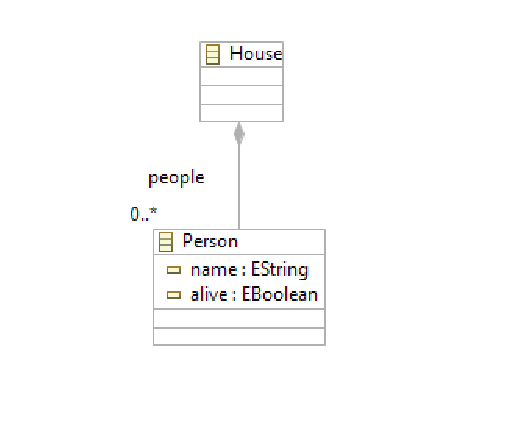
\includegraphics[width=.8\linewidth]{background/images/ejCasa.eps} \\
  \caption{Ejemplo metamodelo casa}
  \label{back:fig:ejMetamodeloCasa}
\end{figure}


Para entender mejor el funcionamiento de EOL se expone el siguiente ejemplo. Se ha definido el meta-modelo mostrado en la figura~\ref{back:fig:ejMetamodeloCasa}, este meta-modelo consiste en la representaci�n de una casa y las personas que viven en ella. Las personas tienen un nombre y un atributo booleano que representa si una persona est� viva o no. Existe una relaci�n de agregaci�n para reflejar que la casa contiene personas.
Una vez creado el meta-modelo podemos crear un modelo como instancia de ese meta-modelo. Un ejemplo de c�mo funciona EOL puede ser el siguiente: deseamos saber que personas habitan en la casa y est�n vivas. La sintaxis correspondiente ser�a la siguiente (figura~\ref{back:code:codigoEOL}).

\begin{figure}[!tb]
\begin{center}
\begin{footnotesize}
\begin{verbatim}
--------------------------------------------------------
for (person in Person.all){
  if (person.alive == true) {
    person.name.println();
  }
}

//Podemos realizar lo mismo de la siguiente manera:

Person.all.select(r|r.alive==true).name.println();

--------------------------------------------------------
\end{verbatim}
\end{footnotesize}
\end{center}
\caption{Ejemplo c�digo EOL}
\label{back:code:codigoEOL}
\end{figure}


Como vemos la sintaxis es muy similar a cualquier lenguaje orientado a objetos, podemos manipular y consultar los objetos del modelo, sin embargo EOL no nos permite la definici�n de clases.


\subsection{Epsilon Transformation Language}
\emph{Epsilon Transformation Language} (ETL) es un lenguaje de transformaci�n modelo a modelo basado en reglas (\imp{Model to Model-M2M}). ETL proporciona las caracter�sticas est�ndar de un lenguaje de transformaci�n, tambi�n nos permite manipular los modelos de entrada y salida as� como su c�digo fuente. ETL tiene su propia sintaxis sin embargo utiliza el lenguaje EOL como base.


Recordando el ejemplo de la Red de computadores y el Grafo detallado en el capitulo anterior (secci�n 1.2). Deseamos realizar la transformaci�n de un modelo de tipo grafo a un modelo de tipo red para ello definiremos una serie de reglas de transformaci�n utilizando para ello ETL. En primer lugar necesitamos definir el modelo del grafo para poder realizar la transformaci�n a un modelo de tipo Red.
La figura~\ref{back:code:codigoETL} muestra el c�digo que realiza el proceso de transformaci�n de un Grafo a una Red.

\begin{figure}[!tb]
\begin{center}
\begin{footnotesize}
\begin{verbatim}

rule Arista2Cable
transform a : Grafo!Arista
to r : Red!Cable {	
    r.nameCable = a.nombreArista;
    if (a.parent.isDefined()) {
        r.parent=Red;
        for (nodoArista in a.children) {
            if(nodoArista.color=TColor#R){
                var PC : new Red!PC;
                PC.nameNodo="PC"+iPC;
                r.children.add(PC);
                iPC=iPC+1;	
            }
            else{
                var Router : new Red!Router;
                Router.nameNodo="Router"+iRouter;
                r.children.add(Router);
                iRouter=iRouter+1;
            }
        }
    }	
}

\end{verbatim}
\end{footnotesize}
\end{center}
\caption{Ejemplo c�digo ETL}
\label{back:code:codigoETL}
\end{figure}

En este c�digo encontramos solo una regla. Esta regla transforma aristas del grafo a cables de la red. La primera instrucci�n copia el nombre de la arista al cable. A continuaci�n la primera condicional cuestiona si esa arista tiene un padre definido en caso afirmativo asigna el cable a la red. A continuaci�n por cada nodo se crea o bien un PC o un router dependiendo del color del nodo que se est� analizando (rojo-PC, azul-Router). En siguiente lugar se asigna el nodo creado al cable correspondiente y finalmente se a�ade a la red. Este proceso se repite por cada arista del grafo. Una vez ejecutado este c�digo dado un modelo de entrada de tipo Grafo obtenemos un modelo equivalente de tipo Red que cumple las reglas definidas en el meta-modelo.


\subsection{Epsilon Generation Language}

\emph{Epsilon Generation Language} (EGL) (\cite{louis:2008}) es un lenguaje utilizado para la generaci�n de c�digo basado en la transformaci�n de modelos (\imp{Model to Text-M2T}).
EGL puede ser utilizado para transformar modelos en cualquier tipo de lenguaje, por ejemplo c�digo ejecutable Java, c�digo HTML o incluso aplicaciones completas que comprenden el c�digo en varios lenguajes (por ejemplo, HTML, Javascript y CSS). En este proyecto se utilizara EGL para la generaci�n de c�digo Cassandra Query Language (CQL) a partir de modelos UML 2.0.

Cada plantilla de EGL contiene varias secciones. Cada secci�n puede ser est�tica o bien din�mica.
Una secci�n est�tica contiene texto que aparecer� en la salida generada por la plantilla. Una secci�n din�mica comienza con la secuencia '[\%' y termina con la secuencia '\%]'. La secci�n din�mica contiene lenguaje EOL.
La figura~\ref{back:code:codigoEGL} muestra como se realiza la generaci�n de c�digo HTML utilizando para ello el modelo generado de una red a partir de un grafo (ver secci�n anterior).

\begin{figure}[!tb]
\begin{center}
\begin{footnotesize}
\begin{verbatim}
--------------------------------------------------------
[%
    var red: Red := Red.allInstances().at(0);
%]

<html>
    <head>
        <title> Red </title>
    </head>
    <body>
        <h1>Conexiones</h1>				
        <table  border="1">
            <col style="width: 200px" />
            <col style="width: 100px" span="3" />
            [% for (conexiones in red.conexiones){%]
            <tr>
                <th scope="row">[%=conexiones.nameCable%]</th>
                [% for (nodos in conexiones.children){%]
                    <td>[%=nodos.nameNodo%]</td>
                [%	}%]
            </tr>
            [%	}%]
        </table>
    </body>
</html>
--------------------------------------------------------
\end{verbatim}
\end{footnotesize}
\end{center}
\caption{Ejemplo c�digo EGL}
\label{back:code:codigoEGL}
\end{figure}

Como vemos en el c�digo la integraci�n del c�digo EGL junto con HTML es total, en este sencillo c�digo se genera una p�gina HTML con una tabla que muestra varias filas, una fila por cada conexi�n entre dos componentes de la red. 

\section{Planificaci�n}
\label{sec:back:planificacion}

%%==================================================================%%
%% Author : Sa�udo Olmedo, Ignacio                                  %%
%%          S�nchez Barreiro, Pablo                                 %%
%% Version: 1.2, 18/06/2013                                         %%
%%                                                                  %%
%% Memoria del Proyecto Fin de Carrera                              %%
%% Background/Planificacion                                         %%
%===================================================================%%

El objetivo de este proyecto de fin de carrera es la implementaci�n de un generador de c�digo Cassandra a partir de modelos UML. El proceso de desarrollo as� como el de aprendizaje que se ha seguido para la realizaci�n del proyecto es descrito a continuaci�n.

La primera tarea como es evidente consisti� en adquirir los conocimientos necesarios para el desarrollo del proyecto, en primer lugar todo lo relacionado con el proceso de modelado de un lenguaje y transformaci�n de lenguajes [kleppe]. Tambi�n fueron necesarios conocimientos sobre la Ingenier�a y el Desarrollo Dirigido por Modelos, as� como de la sintaxis, arquitectura y funcionamiento de Cassandra.

A continuaci�n se comenz� a trabajar con la herramienta Epsilon, sus lenguajes EOL, EGL, ETL y EUnit como herramienta para las pruebas de los modelos y c�digo generados. As� como con el lenguaje para la definici�n de lenguajes de modelado Eclipse Modeling Framework (EMF).
Para conocer c�mo funcionaban estos lenguajes se desarrollaron una serie de casos pr�cticos para familiarizarse con los m�todos de transformaci�n as� como con la herramienta, para ello se realizo el proceso completo para crear un generador de c�digo desde la transformaci�n entre modelos hasta la transformaci�n modelo-c�digo. Estos casos de prueba son los que se exponen en la secci�n de Epsilon.

Una vez conocido estos conceptos se estudiaron las reglas de transformaci�n a aplicar para transformar un modelo UML a un modelo Cassandra, estas reglas fueron propuestas por [pabloCassandra].

Tras estas tareas de adquisici�n de conocimientos se empez� a trabajar en el generador de c�digo Cassandra empezando por la transformaci�n de modelos UML a modelos Cassandra. Estas transformaciones son expuestas en el siguiente cap�tulo. Una vez finalizada la transformaci�n se comenz� a trabajar en el generador de c�digo Cassandra, esta tarea es descrita en el cap�tulo 5. Tras realizar dicha tarea se realizaron una serie de casos de prueba para verificar si los resultados que otorgaba el generador de c�digo eran los esperados, para esta tarea utilizamos la herramienta EUnit.

Finalmente y tras generar varios casos de ejemplo se instalo la plataforma de Cassandra BLABLA 

\section{Sumario}
\label{sec:back:sumario}

%%==================================================================%%
%% Author : Abascal Fern�ndez, Patricia                             %%
%%          S�nchez Barreiro, Pablo                                 %%
%% Version: 1.1, 21/06/2013                                         %%
%%                                                                  %%
%% Memoria del Proyecto Fin de Carrera                              %%
%% Antecedentes, Sumario                                            %%
%%==================================================================%%

Durante este cap�tulo se han descrito los conceptos necesarios para comprender el �mbito y el alcance de este proyecto. Se ha descrito el caso de estudio que se utilizar� a lo largo del documento. A continuaci�n, se ha especificado qu� es una l�nea de productos software, el dise�o orientado a caracter�sticas, la metodolog�a TENTE, las limitaciones de las clases parciales en C\#, c�mo pueden resolverse estas limitaciones mediante el uso del \emph{SlicerPattern} y el proceso de generaci�n de c�digo con Epsilon.

